\section{Explorative Datenanalyse}

\begin{defi}{Explorative Datenanalyse}
    Die \emph{explorative Datenanalyse (EDA)}, eine Weiterentwicklung der deskriptiven Statistik zur Analyse von Daten, arbeitet mehr induktiv: Mit ihren Methoden soll Neues entdeckt, sollen Vermutungen generiert, Besonderheiten erkannt und Sachverhalte dargestellt werden.

    Sie untersucht und begutachtet Daten, von denen nur ein geringes Wissen über deren Zusammenhänge vorliegt. Viele EDA-Techniken werden im Data-Mining eingesetzt.

    Ziele der explorativen Datenanalyse sind:
    \begin{itemize}
        \item Annahmen (\emph{Hypothesen}) über die Ursache und den Grund der beobachteten Daten zu bilden
        \item Annahmen \emph{einzuschätzen}, worauf statistische Inferenz basieren kann
        \item Die Auswahl von passenden statistischen \emph[Werkzeugen und Techniken] zu unterstützen
    \end{itemize}

    \centering
    \includegraphics[width=.9\textwidth]{includes/figures/defi_explorative_datenanalyse.pdf}
\end{defi}

\subsection{Lageparameter}

\begin{defi}{Arithmetisches Mittel}
    Das \emph{arithmetische Mittel} berechnet man, indem man die Summe der betrachteten Zahlen durch ihre Anzahl teilt und beschreibt damit das Zentrum einer Verteilung durch einen numerischen Wert und stellt einen Lageparameter dar.

    Es gilt:
    \begin{itemize}
        \item Für Stichproben in einer Urliste, wobei $x_i$ die Ausprägung des $i$-ten Elements darstellt:
              \[
                  \conj{x} = \frac{1}{n} \sum_{i=1}^n x_i
              \]
        \item Für eine unklassierte Häufigkeitstabelle, wobei $h_i$ die relative Häufigkeit des $i$-ten Elements $a_i$ darstellt:
              \[
                  \conj{x} = \sum_{i=1}^n h_i \cdot a_i
              \]
        \item Für eine klassierte Häufigkeitstabelle, wobei $h_i$ die relative Häufigkeit der $i$-ten Klasse $A_i$, und $\alpha_i$ die Klassenmitte darstellt:
              \[
                  \conj{x} \approx \sum_{i=1}^n h_i \cdot \alpha_i
              \]
    \end{itemize}
\end{defi}

\begin{bonus}{Median}
    Der \emph{Median} der Messwerte einer Urliste ist derjenige Messwert, der genau \enquote{in der Mitte} steht, wenn man die Messwerte der Größe nach sortiert.

    Im Allgemeinen teilt ein Median einen Datensatz, eine Stichprobe oder eine Verteilung so in zwei gleich große Teile, dass die Werte in der einen Hälfte nicht größer als der Medianwert sind und in der anderen nicht kleiner.

    Es gilt:
    \begin{itemize}
        \item Für Stichproben in einer \emph{sortierten} Urliste, wobei $x_i$ die Ausprägung des $i$-ten Elements darstellt:
              \[
                  \tilde{x} =
                  \begin{cases}
                      x_{\nicefrac{(n+1)}{2}}                                                  & \text{falls $n$ ungerade} \\
                      \frac{1}{2} \left( x_{\nicefrac{n}{2}} + x_{\nicefrac{(n+1)}{2}} \right) & \text{falls $n$ gerade}
                  \end{cases}
              \]
        \item Für eine unklassierte Häufigkeitstabelle, wobei $H_i$ die kumulierte relative Häufigkeit bis zum $i$-ten Element $a_i$ darstellt:
              \begin{itemize}
                  \item $\tilde{x}$ ist das Merkmal $a_i$, bei dem $H_i = 0.5$ zum ersten Mal überschritten wird.
              \end{itemize}
        \item Für eine klassierte Häufigkeitstabelle, wobei $H_i$ die kumulierte relative Häufigkeit bis zur $i$-ten Klasse $A_i$ darstellt:
              \begin{itemize}
                  \item $\tilde{x}$ befindet sich in der \emph{Einfallsklasse}, die zum ersten Mal $H_i = 0.5$ erreicht.
                  \item Sei $A_j = \left( a_j, b_j \right]$ die Einfallsklasse.
                        Dann gilt:\footnote{Siehe \emph{Quantil (empirisch)} für mehr Informationen.}
                        \[
                            \tilde{x} = x_{0.5} = a_j + \frac{0.5 - H_{j-1}}{H_{j} - H_{j-1}} \cdot (b_j - a_j)
                        \]
              \end{itemize}
    \end{itemize}
\end{bonus}

\begin{defi}{Quantil (empirisch)}
    Für jede Zahl $p$ zwischen 0 und 1 teilt ein \emph{empirisches p-Quantil} die Stichprobe so, dass ein Anteil der Stichprobe von $p$ kleiner als das empirische $p$-Quantil ist und ein Anteil von $1-p$ der Stichprobe größer als das empirische $p$-Quantil ist.

    Es gilt:
    \begin{itemize}
        \item Für Stichproben in einer \emph{sortierten} Urliste, wobei $x_i$ die Ausprägung des $i$-ten Elements darstellt:
              \[
                  x_p =
                  \begin{cases}
                      \frac{1}{2} \left( x_{n \cdot p} + x_{n \cdot p + 1} \right) & \text{falls $n \cdot p$ ganzzahlig}       \\
                      x_{\floor{n \cdot p + 1}}                                    & \text{falls $n \cdot p$ nicht ganzzahlig} \\
                  \end{cases}
              \]
        \item Für eine unklassierte Häufigkeitstabelle, wobei $h_i$ die relative Häufigkeit des $i$-ten Elements $a_i$ darstellt:
              \begin{itemize}
                  \item $x_p$ ist das Merkmal $a_i$, bei dem $H_i = p$ zum ersten Mal überschritten wird.
              \end{itemize}
        \item Für eine klassierte Häufigkeitstabelle, wobei $H_i$ die kumulierte relative Häufigkeit bis zur $i$-ten Klasse $A_i$ darstellt:
              \begin{itemize}
                  \item $x_p$ befindet sich in der \emph{Einfallsklasse}, die zum ersten Mal $H_i = p$ erreicht.
                  \item Sei $A_j = \left( a_j, b_j \right]$ die Einfallsklasse.
                        Dann gilt:
                        \[
                            x_p = a_j + \frac{p - H_{j-1}}{H_{j} - H_{j-1}} \cdot (b_j - a_j)
                        \]
              \end{itemize}
    \end{itemize}
\end{defi}

\subsection{Streuungsparameter}

\begin{defi}{Empirische Varianz}
    Die \emph{empirische Varianz} bzw. \emph{Stichprobenvarianz}  ist eine statistische Angabe für die Streubreite von Werten einer Stichprobe.

    Sie gehört zu den Streuungsmaßen und beschreibt die mittlere quadratische Abweichung der einzelnen Messwerte vom empirischen Mittelwert.

    Sie stellt damit eine Art durchschnittliches Abweichungsquadrat dar.

    Die positive Wurzel der empirischen Varianz ist die \emph{empirische Standardabweichung}.
    Die empirische Standardabweichung stellt das gebräuchlichste Streuungsmaß dar.

    Es gilt:
    \begin{itemize}
        \item Für Stichproben in einer Urliste, wobei $x_i$ die Ausprägung des $i$-ten Elements darstellt:
              \[
                  s^2 = \frac{1}{n-1} \sum_{i=1}^{n} (x_i - \conj{x})^2 = \frac{1}{n-1} \left( \sum_{i=1}^{n} x_i^2 - n\cdot \conj{x}^2 \right)
              \]
        \item Für eine unklassierte Häufigkeitstabelle, wobei $n_j$ die absolute Häufigkeit des $j$-ten Elements $a_j$ darstellt:
              \[
                  s^2 = \frac{1}{n-1} \sum_{j=1}^{m} (a_j - \conj{x})^2 \cdot n_j = \frac{1}{n-1} \left( \sum_{j=1}^{m} a_j^2 \cdot n_j - \conj{x}^2 \right)
              \]
        \item Für eine klassierte Häufigkeitstabelle, wobei $n_j$ die absolute Häufigkeit der $j$-ten Klasse $A_j$, und $\alpha_j$ die Klassenmitte darstellt:
              \[
                  s^2 \approx \frac{1}{n-1} \sum_{j=1}^{m} \alpha_j^2 \cdot n_j - \frac{1}{n(n-1)} \left( \sum_{j=1}^{m} \alpha_j \cdot n_j \right)^2
              \]
    \end{itemize}

    Insgesamt gilt natürlich jeweils für die empirische Standardabweichung:
    \[
        s = \sqrt{s^2}
    \]
\end{defi}

\begin{defi}{Quartilsabstand}
    Der \emph{Quartilsabstand} bzw. \emph{Interquartilsabstand} $Q$ gibt für eine sortierte Stichprobe an, wie breit das Intervall ist, in dem die mittleren 50\% der Stichprobeelemente liegen.

    Es gilt:
    \[
        Q = x_{0.75} - x_{0.25}
    \]
\end{defi}

\subsection{Deskriptive Statistik}

\begin{defi}{Box-Plot}
    \begin{wrapfigure}{r}{0.5\textwidth}
        \centering
        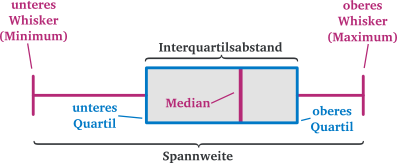
\includegraphics[width=0.45\textwidth]{includes/figures/definition_boxplot.png}
    \end{wrapfigure}%
    %
    Der \emph{Box-Plot} ist ein Diagramm, das zur grafischen Darstellung der Verteilung eines mindestens ordinalskalierten Merkmals verwendet wird.

    Es fasst dabei verschiedene robuste Streuungs- und Lagemaße in einer Darstellung zusammen.

    Ein Box-Plot soll schnell einen Eindruck darüber vermitteln, in welchem Bereich die Daten liegen und wie sie sich über diesen Bereich verteilen. Deshalb werden alle Werte der sogenannten Fünf-Punkte-Zusammenfassung, also der Median, die zwei Quartile und die beiden Extremwerte, dargestellt.

    Zusammengefasst lassen sich folgende Kennwerte ablesen:

    \begin{center}
        \begin{tabular}{|l|p{0.4\linewidth}|p{0.3\linewidth}|}
            \hline
            Kennwert        & Beschreibung                                                                          & Lage im Box-Plot                                   \\
            \hline
            \hline
            Minimum         & Kleinster Datenwert des Datensatzes                                                   & Ende eines Whiskers oder entferntester Ausreißer   \\
            \hline
            Unteres Quartil & Die kleinsten 25\% der Datenwerte sind kleiner als dieser oder gleich diesem Kennwert & Beginn der Box                                     \\
            \hline
            Oberes Quartil  & Die kleinsten 75\% der Datenwerte sind kleiner als dieser oder gleich diesem Kennwert & Ende der Box                                       \\
            \hline
            Maximum         & Größter Datenwert des Datensatzes                                                     & Ende eines Whiskers oder entferntester Ausreißer   \\
            \hline
            Spannweite      & Gesamter Wertebereich des Datensatzes                                                 & Länge des gesamten Box-Plots (inklusive Ausreißer) \\
            \hline
            Quartilsabstand & Wertebereich, in dem sich die mittleren 50\% der Daten befinden                       & Ausdehnung der Box                                 \\
            \hline
        \end{tabular}
    \end{center}
\end{defi}

\begin{bonus}{5 Number Summary}
    TODO
\end{bonus}

\begin{defi}{Histogramm}
    TODO
\end{defi}

\subsection{Visualisierung}

\begin{defi}{Regeln für Visualisierungen}
    Regeln nach Edward Tufte:
    \begin{itemize}
        \item Maximieren des Daten-Druckerschwärze-Verhältnis (so wenig Druckerschwärze für soviele Daten wie möglich)
        \item Minimieren des Lügenfaktors
        \item Minimieren des \enquote{Chartjunks} (keine visuellen Spielereien)
        \item Nutzen von angemessenen Skalen, Achsenbeschriftungen
        \item Farbe zum Darstellen von Eigenschaften der Daten, nicht für Ästhetik oder Kommunikation
    \end{itemize}
\end{defi}

\begin{bonus}{Notwendigkeit von Visualisierungen}
    Für unterschiedliche Datensätze können ähnliche Kennzahlen entstehen.

    Aus diesem Grund werden Visualisierungen für die Erkundung von Daten benötigt.
\end{bonus}

\begin{bonus}{Auswahl einer Diagrammart}
    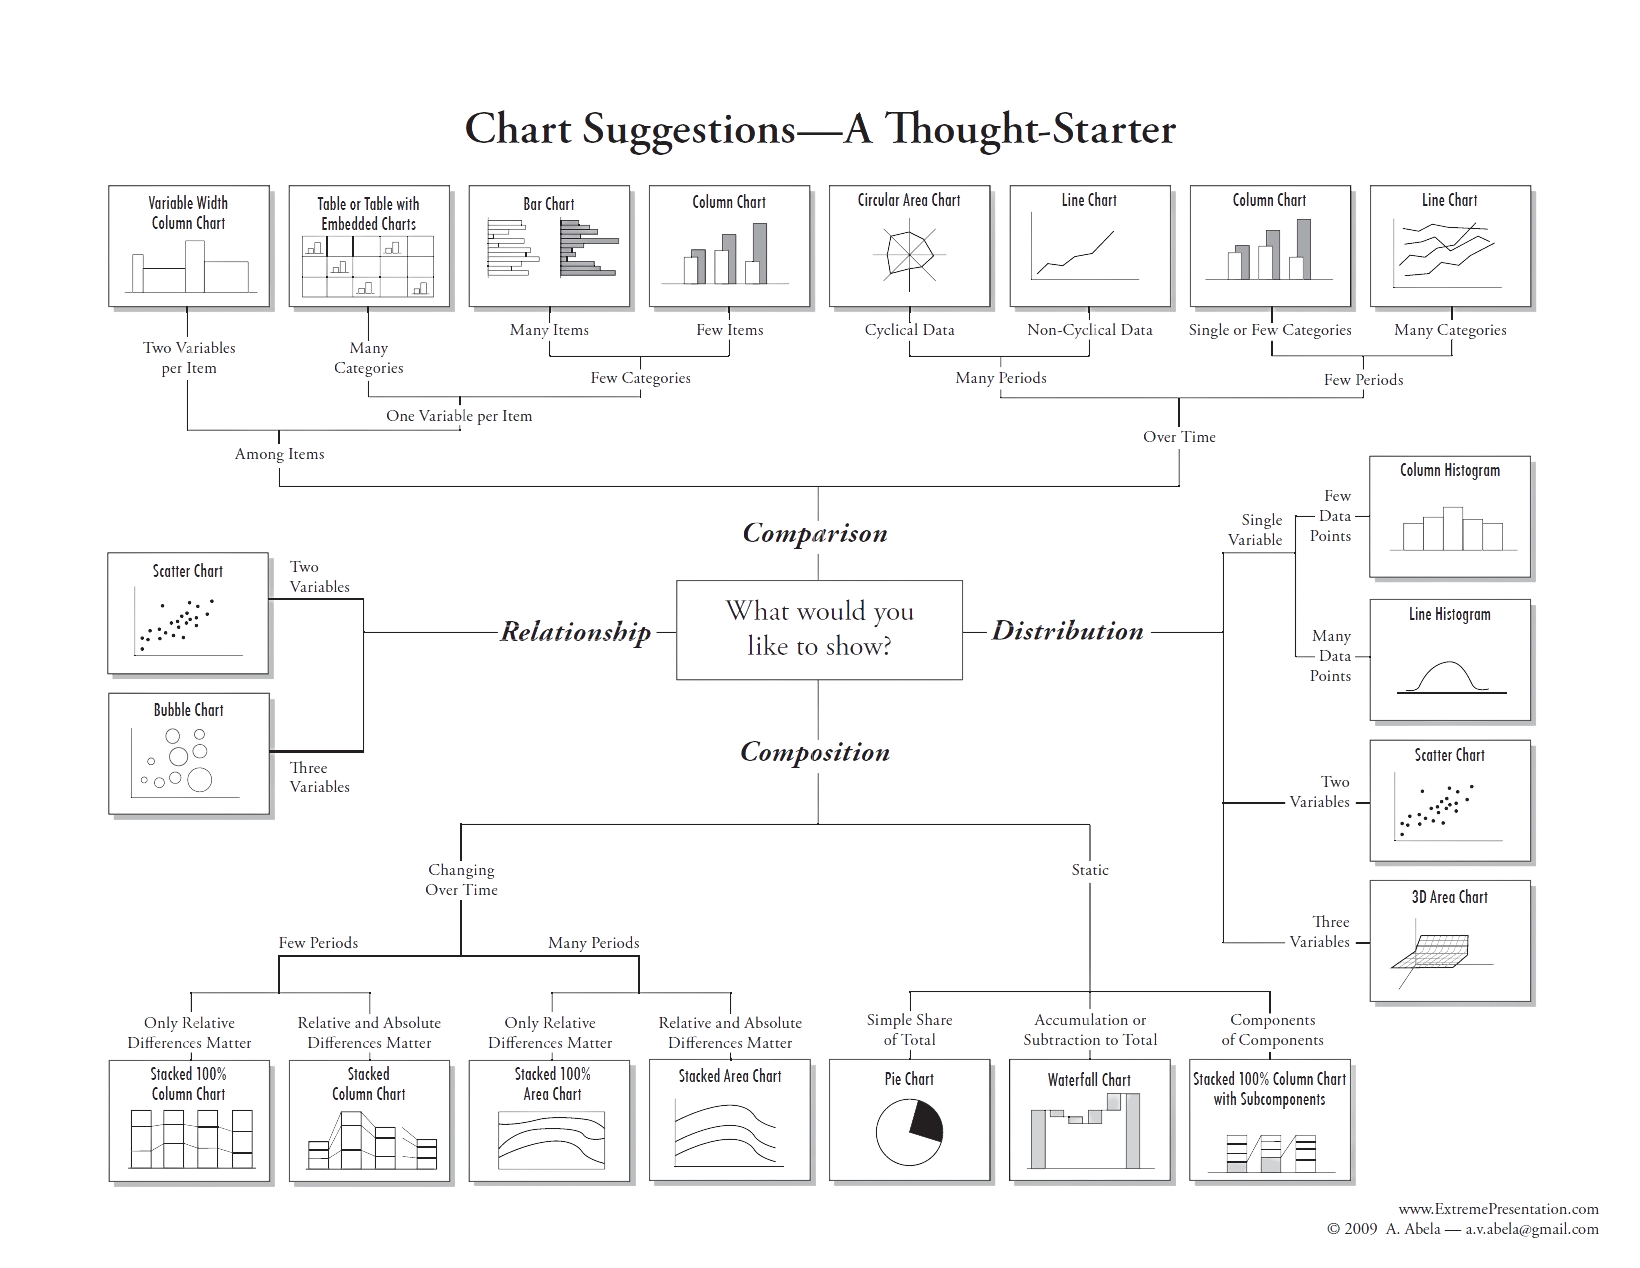
\includegraphics[width=\textwidth]{includes/figures/bonus_chart_suggestion.png}
\end{bonus}

\begin{example}{Anscombe-Quartett}
    Das \emph{Anscombe-Quartett} besteht aus vier Mengen von Datenpunkten, die nahezu identische einfache statistische Eigenschaften haben, aber aufgetragen sehr verschieden aussehen.

    Für die vier Punktmengen gilt:
    \begin{itemize}
        \item Mittelwert von $x$ in jedem Fall: 9 (exakt)
        \item Varianz von $x$ in jedem Fall: 11 (exakt)
        \item Mittelwert von $y$ in jedem Fall: 7.50 (auf 2 Stellen)
        \item Varianz von $y$ in jedem Fall: 4.122 oder 4.127 (auf 3 Stellen)
        \item Korrelation zwischen $x$ und $y$ in jedem Fall: 0.816 (auf 3 Stellen)
        \item Lineare Regression in jedem Fall: $y = 3.00 + 0.500x$ (auf 2 bzw. 3 Stellen)
    \end{itemize}

    Die Datenpunkte sind gegeben wie folgt:

    \begin{center}
        \begin{tabular}{|l|l||l|l||l|l||l|l|}
            \hline
            \multicolumn{2}{|l||}{Reihe 1} & \multicolumn{2}{l||}{Reihe 2} & \multicolumn{2}{l||}{Reihe 3} & \multicolumn{2}{l|}{Reihe 4}                               \\ \hline
            x                              & y                             & x                             & y                            & x    & y     & x    & y     \\ \hline\hline
            4.0                            & 4.26                          & 4.0                           & 3.10                         & 4.0  & 5.39  & 8.0  & 5.25  \\ \hline
            5.0                            & 5.68                          & 5.0                           & 4.74                         & 5.0  & 5.73  & 8.0  & 5.56  \\ \hline
            6.0                            & 7.24                          & 6.0                           & 6.13                         & 6.0  & 6.08  & 8.0  & 5.76  \\ \hline
            7.0                            & 4.82                          & 7.0                           & 7.26                         & 7.0  & 6.42  & 8.0  & 6.58  \\ \hline
            8.0                            & 6.95                          & 8.0                           & 8.14                         & 8.0  & 6.77  & 8.0  & 6.89  \\ \hline
            9.0                            & 8.81                          & 9.0                           & 8.77                         & 9.0  & 7.11  & 8.0  & 7.04  \\ \hline
            10.0                           & 8.04                          & 10.0                          & 9.14                         & 10.0 & 7.46  & 8.0  & 7.71  \\ \hline
            11.0                           & 8.33                          & 11.0                          & 9.26                         & 11.0 & 7.81  & 8.0  & 7.91  \\ \hline
            12.0                           & 10.84                         & 12.0                          & 9.13                         & 12.0 & 8.15  & 8.0  & 8.47  \\ \hline
            13.0                           & 7.58                          & 13.0                          & 8.74                         & 13.0 & 12.74 & 8.0  & 8.84  \\ \hline
            14.0                           & 9.96                          & 14.0                          & 8.10                         & 14.0 & 8.84  & 19.0 & 12.50 \\ \hline
        \end{tabular}
    \end{center}

    Die Reihen sind offensichtlich komplett verschieden:

    \centering
    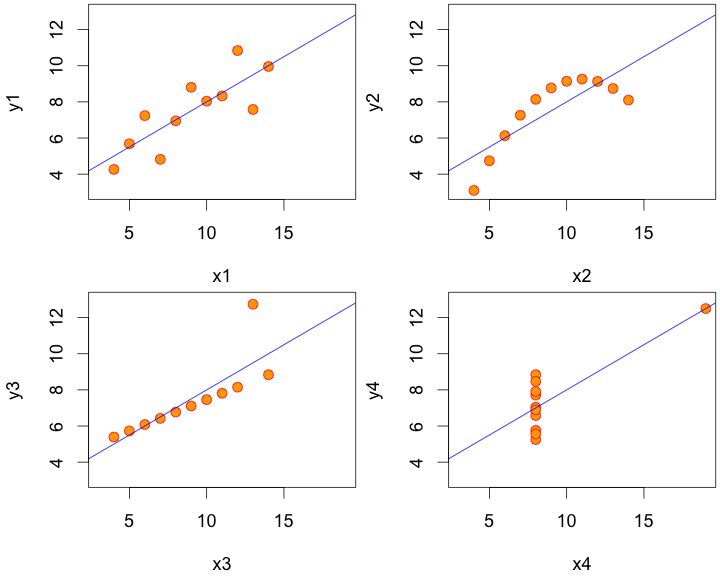
\includegraphics[width=.7\textwidth]{includes/figures/example_anscombe.png}
\end{example}